\section{\texorpdfstring{\LaTeX}{LaTeX}-Beispiele%
         \label{sec:LaTeX-Beispiele}}

Dieser Abschnitt soll einen schnellen Start zum Schreiben einer
wissenschaftlichen Arbeit mit Hilfe von \LaTeX\ am CVH ermöglichen. 
Daher finden sich in diesem Abschnitt im Wesentlichen Beispiele für die
wichtigsten Textobjekte innerhalb wissenschaftlicher Arbeiten. 
Für weiterführende Dokumentationen sei auf die umfassende Zahl an Büchern und
Internetdokumenten verwiesen (hier kommen noch Verweise hin!!!!!!!!!). 

\subsection{Compilieren%
            \label{sec:Compilieren}}

Diese Datei wurde ursprünglich mit PDF\LaTeX\ in der Umgebung Kile unter GNU/Linux compiliert.
Es sind die Pakete \file{texlive-lang-german} und \file{texlive-latex-extra} erforderlich.
  % Der Befehl \file{...} wird in hauptdatei.tex definiert.
  % Siehe dort.
Eventuell sind weitere Pakete zu installieren.
    
Beim Compilieren kann(!) die Warnung %\enquote{destination with the same identifier}
\glqq{}destination with the same identifier\grqq{}
gemeldet werden. Diese dürfen Sie ignorieren.
  % @@@ PG: Wirklich? Warum? Was ist da los? Bei mir tritt sie übrigens nicht auf.

\subsection{Abschnitte und Unterabschnitte%
            \label{sec:Abschnitte}}

Dies (\glqq{}{\ref{sec:Abschnitte}.~Abschnitte und Unterabschnitte}\grqq{})
ist ein Unterabschnitt des Abschnitts \glqq{}{\ref{sec:LaTeX-Beispiele}.~\LaTeX-Beispiele}\grqq{}.
Der Befehl \lstinline|\section| generiert einen Abschnitt und
der Befehl \lstinline|\subsection| einen Unterabschnitt.

\subsubsection{Unter-Unterabschnitte%
               \label{sec:Unter-Unterabschnitte}}

Diese weitere Untergliederung geschieht mit dem Befehl \lstinline|\subsubsection|.

Eine noch weitere Untergliederung in eine vierte oder noch tiefere Ebene ist zu
vermeiden (und in \LaTeX\ normalerweise auch nicht vorgesehen).
 
\subsection{Bilder und Tabellen%
            \label{sec:Bilder-Tabellen}}

In wissenschaftlichen Arbeiten bilden der Text und die Abbildungen keine Einheit.
Abbildungen sind vielmehr eigenständige Objekte, die unabhängig vom Text positioniert werden.
Sie \glqq{}{gleiten}\grqq{} gewissermaßen durch den Text
und werden daher im Englischen als \glqq{}{floats}\grqq{} bezeichnet.

\LaTeX\ hilft dabei, für alle gleitenden Objekte
-- Abbildungen, Tabellen, Programmquelltexte usw.\ -- 
den jeweils besten Platz im Dokument zu finden.
Dies kann oben oder unten auf der aktuellen Seite sein,
auf einer separaten Seite oder auch, wenn die Möglichkeit besteht,
zwischen Absätzen im Text.

Gleitende Objekte tragen Nummern, auf die sich der Text bezieht.
Die folgenden Abschnitte zeigen dies anhand von Beispielen.

\subsubsection{Bilder%
               \label{sec:Bilder}}

Bild \ref{fig:roll_pitch_yaw} ist ein Beispielbild,
das auf Seite~\pageref{fig:roll_pitch_yaw} steht.

% Es folgt eine einfache Anwendung für „Programmierung“ mit \ifthenelse:
%
% Wenn die beiden referenzierten Abbildungen auf derselben Seite sind,
% lautet der Text: „..., das auf Seite x steht. Ebenfalls auf Seite x ...“
% Ansonsten lautet er: „..., das auf Seite x steht. Auf Seite y ...“
%
\ifthenelse{\equal{\pageref{fig:roll_pitch_yaw}}{\pageref{fig:quadrocopter}}}%
           {Ebenfalls auf}%
           {Auf}
Seite~\pageref{fig:quadrocopter} stehen mehrere Bilder
(\ref{fig:quadrocopter} und \ref{fig:ka32S}) nebeneinander.

% Mit \begin{figure} ... \end{figure} wird das Bild in einen
% „gleitenden Kasten“ (engl.: „float“) eingeschlossen,
% der unabhängig vom Text positioniert wird.
%
% Das große H in eckigen Klammern besagt, daß das Bild „hier“ im
% Text erscheinen soll. Möglich ist:
%   H – auf jeden Fall hier
%   h – hier, wenn es möglich ist
%   t – oben auf einer Seite
%   b – unten auf einer Seite
%   p – auf einer separaten Seite
% Diese verschiedenen Möglichkeiten können auch als erste, zweite,
% dritte Wahl usw. hintereinandergeschrieben werden.
%
\begin{figure}[H]
  \begin{center}
    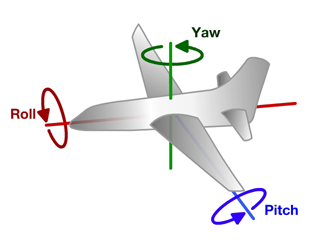
\includegraphics[width=0.3\textwidth]{bilder/roll_pitch_yaw}
      % Einbinden einer Pixelgrafik.
      % Die Endung „.png“ darf weggelassen werden.
    \caption{Ein Beispielbild mit Quellenangabe \citep{yawpitchroll2013}%
             \label{fig:roll_pitch_yaw}}
  \end{center}
\end{figure}

\begin{minipage}[b]{7cm}
  \centering
    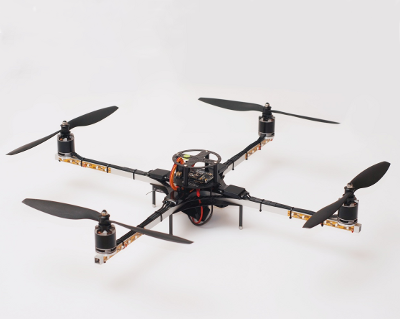
\includegraphics[width=7cm]{bilder/quadrocopter}
    \captionof{figure}{Quadrocopter \newline
                         % kein \\ innerhalb von \caption oder \captionof
                         % \newline
                       \citep{bild_quad}%
	               \label{fig:quadrocopter}}
\end{minipage}\hfill
\begin{minipage}[b]{7cm}
  \centering
  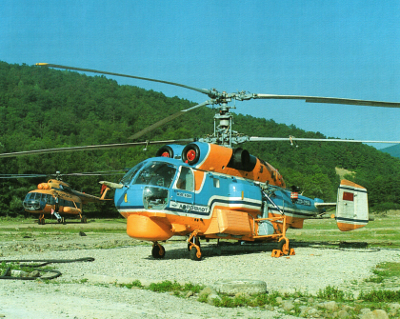
\includegraphics[width=7cm]{bilder/ka32S}
  \captionof{figure}{Koaxialhelicopter \newline
                     \citep[S. 101]{hubschrauber1997}%
                     \label{fig:ka32S}}
\end{minipage}
	
\subsubsection{Tabellen%
               \label{sec:Tabellen}}

\begin{table}[H]
  \caption{Masse des anzuhebenden Trägers%
           \label{table:massen}}
  \medskip
  \begin{center}
    \begin{tabular}{l|r}
      %
      % Die Leerzeichen im Quelltext haben keinen Einfluß auf die
      % Anordnung innerhalb der Tabelle. Diese wird durch die o.a.
      % Angabe „{l|r}“ gesteuert: linksbündiges Feld, senkrechter
      % Strich, rechtsbündiges Feld.
      %
      Bauteil                  & Masse[g] \\
      \hline
      Trägerrohr               &       35 \\
      Linearlager              &        7 \\
      Lagerblock Linearlager   &        5 \\
      Kabel und Schrauben      &       20 \\
      Motoren                  &       50 \\
      Propeller                &       10 \\
      Propeller Eingriffschutz &       80 \\
      Holzplatte               &       14 \\
      Drehzahlsensoren         &        5 \\
      \hline
      Gesamtmasse              &      226 \\
      % @@@ PG: Stimmt nicht: Die Summe der Zahlen ist 194!
    \end{tabular}
  \end{center}
\end{table}

% Mit dem folgenden Befehl teilen wir LaTeX mit, daß wir es für
% besser halten, an dieser Stelle (also vor dem Textabsatz) eine
% neue Seite zu beginnen, als den Textabsatz auf zwei Seiten zu
% verteilen.
%
\goodbreak

Bilder haben Bildunterschriften;
bei Tabellen hingegen sind Überschriften üblich.
Tabelle~\ref{table:massen} zeigt eine Tabelle ohne Umrahmung. 
Demgegenüber zeigt Tabelle~\ref{table:massen_rahmen}
eine Version mit gleichem Inhalt, aber mit Umrahmung. 

\goodbreak

\begin{table}[H]
  \caption{Masse des anzuhebenden Trägers%
           \label{table:massen_rahmen}}
  \medskip
  \begin{center}
    \begin{tabular}{|l|r|}
      \hline
      Bauteil                  & Masse[g] \\
      \hline
      Trägerrohr               &       35 \\
      Linearlager              &        7 \\
      Lagerblock Linearlager   &        5 \\
      Kabel und Schrauben      &       20 \\
      Motoren                  &       50 \\
      Propeller                &       10 \\
      Propeller Eingriffschutz &       80 \\
      Holzplatte               &       14 \\
      Drehzahlsensoren         &        5 \\
      \hline
      Gesamtmasse              &      226 \\
      % @@@ PG: Stimmt nicht: Die Summe der Zahlen ist 194!
      \hline
    \end{tabular}
  \end{center}
\end{table}
    
\subsection{Zitate%
            \label{sec:Zitate}}

Neue Quellen sind in die Datei \file{hauptdatei.bib} einzutragen.
   
\glqq{}{Boris ermöglicht die blockorientierte Simulation
         dynamischer Systeme nahezu beliebiger Art}\grqq{}
         \citep[S. 25]{boris2009}.
         

Möchten Sie nicht eine Seite zitieren sondern Seite 18 und alle folgenden, dann erfolgt das in der Form 
\citep[S. 18ff]{boris2009}.
Meinen Sie tatsächlich jedoch Seite 18 und eine(!) weitere, also Seiten 18 und 19, so findet sich auch oft der Eintrag 
\citep[S. 18f]{boris2009}.
Ein \glqq{}f\grqq{} steht also für eine weitere Seite hinter der Nummer und \glqq{}ff\grqq{} für (viele) weitere Seiten hinter bzw.~ab der Nummer. 

Ein Beispiel für ein Zitat ohne Seitenangabe sieht wie folgt aus: 
\citep{kleinantriebe2011}. 
    
Die Grundausstattung von Simulink unterstützt unter
anderem Arduino-Plattformen und das Raspberry-PI Board
\citep{mathworks2013}.

% @@@ PG: Wieso ist das eine Zitat in Anführungszeichen und das andere nicht?
   
\subsection{Gleichungen%
            \label{sec:Gleichungen}}

Gleichungen erhalten automatisch Nummern, auf die sich der Text beziehen kann.
Beispiel: Gleichungen wie (\ref{eq:drehmoment-1}) und (\ref{eq:drehmoment-2})
beschreiben den Zusammenhang zwischen Leistung, Drehmoment und Drehzahl.

Gleichungen in tabellarischer Form
\begin{eqnarray}
  P_\text{Welle}         &=& 2  \pi  M  n \label{eq:drehmoment-1} \\
  \Leftrightarrow\quad M &=& \frac{P_\text{Welle}}{ 2  \pi  n} \label{eq:drehmoment-2}
\end{eqnarray}
%
% Zur manuellen „Verschönerung“ von Gleichungen kann man
% verschiedene Formen von Leerzeichen einsetzen:
% \,     – halbes Leerzeichen
% ~      – ganzes Leerzeichen
% \quad  – etwa doppelt so breit wie ein Leerzeichen
% \qquad – doppelt so breit wie \quad
% \!     – negatives halbes Leerzeichen
%
werden in einer \lstinline|eqnarray|-Umgebung gesetzt.
Daneben unterstützt \LaTeX\ auch die einfache Standardvariante für
Gleichungen in einer \lstinline|equation|-Umgebung. 
\begin{equation}
  U = R  I ~\Leftrightarrow~ I = \frac{U}{R}
  \label{eq:Ohmsches-Gesetz}
\end{equation}
%
% Hier zum Beispiel wird die zentrale Bedeutung des Äquivalenzsymbols
% durch zusätzliche Leerzeichen hervorgehoben.
Bei eigenen Mitschriften in Vorlesungen schreiben einige Studierende gerne eine Punkt als Multiplikationszeichen zwischen den Formelzeichen, also zum Beispiel $U=R\cdot I$. 
In gedruckter Form ist das unüblich und der Punkt $\cdot $ entfällt.     
    
    
\subsection{Eintrag in die Nomenklatur%
            \label{sec:Nomenklatur}}

Die Abkürzung PWM \nomenclature[A]{PWM}{Pulsweitenmodulation} bedeutet Pulsweitenmodulation. 
Die Option [A] legt das Objekt in den Unterabschnitt Abkürzungen in der Nomenklatur.
    
Das Symbol $\pi$ \nomenclature[S]{$\pi$}{Kreis-Konstante} ist die Kreiskonstante (die reelle Zahl \glqq{}Pi\grqq{}).
Die Option [S] legt das Objekt in den Unterabschnitt Symbole in der Nomenklatur.

MakeIndex zur Erzeugung der Nomenklatur und BibTex zur Erzeugung des Literaturverzeichnis werden aus dem tex-File aufgerufen. Diese Aufrufe geschehen direkt vor \textit{documentclass} in der Datei \textit{hauptdatei.tex}.

\textbf{Eine Konfiguration der Latex-IDE wie im Folgenden beschrieben sollte daher normalerweise nicht notwendig sein.}

Falls die Erzeugung dennoch nicht funktioniert, können die Tools PDFLaTex, BibTex und MakeIndex von Hand nacheinander aufgerufen werden.
Dafür muss MakeIndex in der Latex-IDE jedoch wie folgt konfiguriert werden.

Um die Nomenklatur zu erstellen wird der Befehl \textit{makeindex} verwendet.
Dieser Befehl muss in der Latex-Entwicklungsumgebung (MiKTex, Kile oder andere) richtig konfiguriert werden.
Insbesondere müssen dem Tool \textit{makeindex} die Parameter \textit{-s nomencl.ist -o hauptdatei.nls hauptdatei.nlo} übergeben werden.
Das Vorgehen hierfür hängt von der Entwicklungsumgebung ab und ist im Folgenden für Kile und MiKTeX beschrieben.

\subsubsection*{Kile}
Um die Entwicklungsumgebung Kile für die automatische Generierung der Nomenklatur zu konfigurieren, müssen die Einstellungen gemäß Abbildung \ref{fig:configNomclKile} vorgenommen werden.
Hierzu im Menü Settings -> Configure Kile... -> Tools -> Build -> MakeIndex anwählen.
Anschließend unter Options \textit{-s nomencl.ist -o \%S.nls \%S.nlo} eintragen und mit \textit{OK} bestätigen.
Nun sollte der Aufruf von PDFLaTeX automatisch die Nomenklatur erzeugen.

\begin{figure}[H]
  \begin{center}
    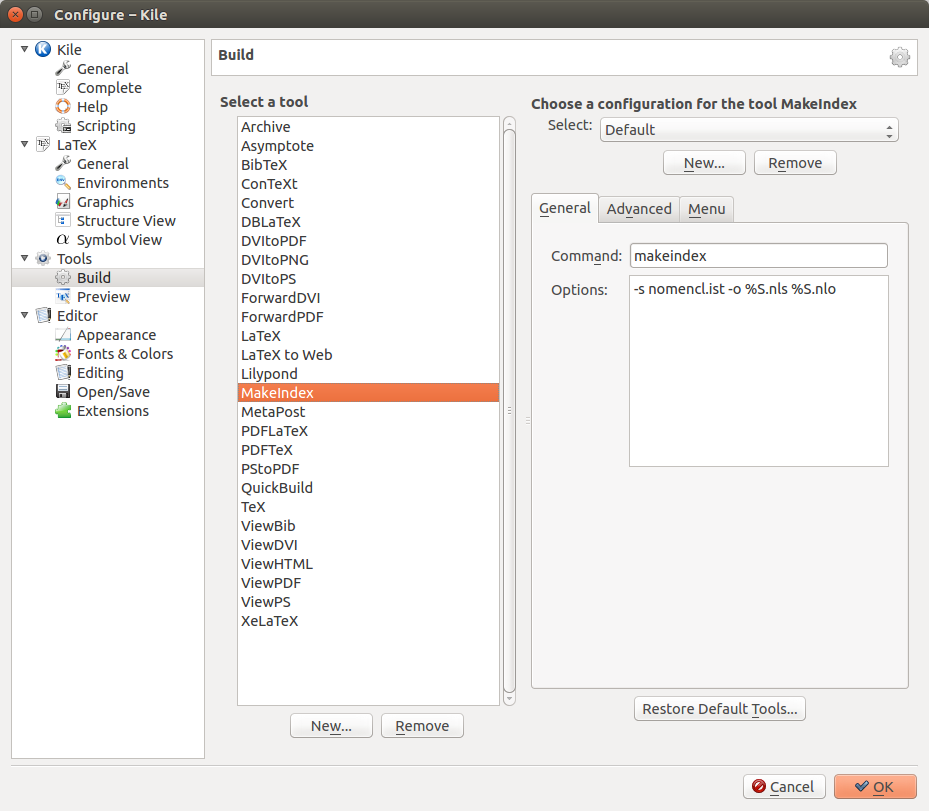
\includegraphics[width=1.0\textwidth]{bilder/configNomclKile}
      % Einbinden einer Pixelgrafik.
      % Die Endung „.png“ darf weggelassen werden.
    \caption{Konfiguration von \textit{makeindex} unter Kile\label{fig:configNomclKile}}
  \end{center}
\end{figure}



\subsubsection*{MiKTeX TeXworks}
Um die Entwicklungsumgebung MiKTeX TeXworks für die automatische Generierung der Nomenklatur zu konfigurieren, müssen die Einstellungen gemäß Abbildung \ref{fig:configNomclMiktex} vorgenommen werden.
Hierzu im Menü Edit -> Preferences... -> Typesetting in der Auswahlbox \textit{Processing tools}  den Eintrag \textit{MakeIndex} anwählen und \textit{Edit} klicken.
In dem erscheinenden Fenster gemäß Abbildung \ref{fig:configNomclMiktex} unter \textit{Arguments} mit dem +Button die fünf Zeilen \textit{-s, nomencl.ist, -o, \$basename.nls, \$basename.nlo} eintragen. 
Hierbei ist die Reihenfolge wichtig.
Um nun die Nomenklatur zu erzeugen muss erst \textit{pdfLaTex}, dann \textit{MakeIndex} und wieder \textit{pdfLaTex} aufgerufen werden.
Der Aufruf von dem Tool \textit{pdfLaTex+MakeIndex+BibTeX} funktioniert nicht, weil hierbei die oben getroffene Konfiguration von MakeIndex nicht umsetzbar ist.
 

\begin{figure}[H]
  \begin{center}
    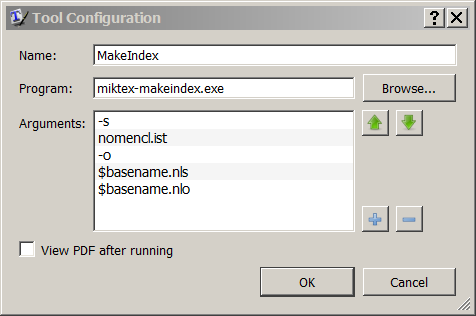
\includegraphics[width=0.6\textwidth]{bilder/configNomclMiktex}
      % Einbinden einer Pixelgrafik.
      % Die Endung „.png“ darf weggelassen werden.
    \caption{Konfiguration von \textit{MakeIndex} unter MiKTeX TeXworks\label{fig:configNomclMiktex}}
  \end{center}
\end{figure}


\subsubsection*{Fehlerbehebung}
Falls \textit{makeindex} die Nomenklatur nicht wie gewünscht erzeugt kann es helfen, das Projektverzeichnis zu bereinigen.
Dies geschieht, indem die automatisch erzeugten Dateien gelöscht werden.
Hierzu zählen insbesondere die Dateien mit den Endungen toc, out, nlo, lot, log, lof, aux, nls, ilg, idx, blg und bbl.

Unter einer älteren Version von MiKTeX wurde zwar eine Nomenklatur erstellt, es gab jedoch keine Beschreibungen zu den einzelnen Einträgen der Nomenklatur.
Die Deinstalltion von MiKTex und Neuinstallation der neuesten Version führte zum Erfolg. 

    
%
% Durch das [language=sh] teilen wir \lstinline mit,
% daß es sich nicht um einen Befehl in der Standard-Sprache (TeX) handelt,
% sondern um einen Befehl in der Unix-Shell-Sprache (sh).
% Dies wird für die automatische Erkennung von Schlüsselwörtern,
% Strings, Kommentaren usw. benötigt. (Hier: „%source ...“ wäre
% sonst ein Kommentar und würde kursiv gesetzt.)
